%\documentclass{beamer} 
\documentclass[handout]{beamer} 
\usetheme{Ilmenau}
\usepackage{graphicx,verbatim,hyperref}
\usepackage{textpos}

\usecolortheme{beaver}
\useinnertheme{default}
\setbeamertemplate{itemize item}[triangle]
\setbeamertemplate{itemize subitem}[triangle]
\setbeamertemplate{itemize subsubitem}[circle]
\setbeamertemplate{enumerate items}[default]
\setbeamertemplate{blocks}[upper=block head,rounded]
\setbeamercolor{item}{fg=black}
\usefonttheme{serif} %should allow ccfonts to take effect

\usepackage{cite}
\usepackage{times, verbatim,xcolor,bm}
%\usepackage[usenames,dvipsnames]{color}
\usepackage{amsbsy,amssymb, amsmath, amsthm}
\usepackage{booktabs}
%David miller's fonts
	\usepackage[T1]{fontenc}
	\usepackage[boldsans]{ccfonts}
	%\usepackage[boldsans]{concmath}
	\usepackage[euler-hat-accent]{eulervm}

\newcommand{\al}{\alpha}
\newcommand{\expect}{\mathbb{E}}
\newcommand{\Bt}{B(\bm{\tau^a})}
\newcommand{\bta}{\bm{\tau^a}}
\newcommand{\btn}{\bm{\tau^{tw}}}
\newcommand{\ga}{\gamma}
\newcommand{\ve}{\varepsilon}
\newcommand{\ta}{\theta}
\newcommand{\de}{\delta}
\newcommand{\ov}{\overline}
\newcommand{\un}{\underline}

\newenvironment{changemargin}[2]{% 
  \begin{list}{}{% 
    \setlength{\topsep}{0pt}% 
    \setlength{\leftmargin}{#1}% 
    \setlength{\rightmargin}{#2}% 
    \setlength{\listparindent}{\parindent}% 
    \setlength{\itemindent}{\parindent}% 
    \setlength{\parsep}{\parskip}% 
  }% 
  \item[]}{\end{list}} 
	
	\let\Tiny=\tiny


\title[Lobbying and Legislative Uncertainty\hspace{2.95in}\insertframenumber/\inserttotalframenumber]{Lobbying and Legislative Uncertainty}
\author[Buzard and Saiegh \hspace{3in} \url{kbuzard@syr.edu}]{Kristy Buzard\inst{1} \and Sebastian Saiegh\inst{2}}
\institute{\inst{1}Syracuse University and The Wallis Institute \and 
\inst{2}UC San Diego}
\date{May 10, 2016}
\begin{document}
\maketitle
%\insertpresentationendpage removed b/c of appendix




\section{Overview}
\subsection{Overview}
\begin{frame}{The Questions}

\pause
\begin{enumerate}[<+->]
\item How does uncertainty about legislators' preferences impact 
	\begin{itemize}
		\item lobbying strategies (e.g. who to lobby, how much to `pay')
		\item probability a bill passes
	\end{itemize}
	\vskip.1in
\item Can we distentangle fundamental uncertainty about preferences from equilibrium and modeling uncertainty?
	\begin{itemize}
		\item[$\Rightarrow$] build a structural model to take to U.S. House data
	\end{itemize}
	\vskip.1in
\item Ultimately, want to identify cross-industry measures of legislative uncertainty
	\begin{itemize}
		\item but for today, unidimensional model
	\end{itemize}
\end{enumerate}

\end{frame}

\begin{frame}{Literature}
\pause
\begin{itemize}[<+->]
	\item \textbf{Probabilistic Voting with Policy Motivation}: Roemer 1994, 1997, Duggan $\&$ Fey 2011
	\item \textbf{Lobbying with Uncertainty}: Coates $\&$ Ludema 2001, Le Breton $\&$ Salanie 2003, Le Breton $\&$ Zaphorozhets 2007
	\item \textbf{Vote Buying in Legislatures}: Groseclose $\&$ Snyder 1996, Banks 2000, Dal Bo 2007
	\item \textbf{Influence w/out Vote Buying}: Fox $\&$ Rothenberg 2011
\end{itemize}
\end{frame} 



\begin{frame}{Some Stylized Facts}

\pause
\begin{enumerate}[<+->]
	\item In the U.S., about $\$ 4$ billion / yr spent on lobbying and campaign contributions
	\item There is usually lobbying on both sides of a given issue
	\item Moderate legislators receive more contributions than those that are ideologically extreme
	\item Legislators about whom there is a moderate level of uncertainty are lobbied the most
\end{enumerate}

\pause
\vskip.2in
Adding uncertainty to standard model captures (2) --- (4)
\end{frame}


%\begin{frame}
%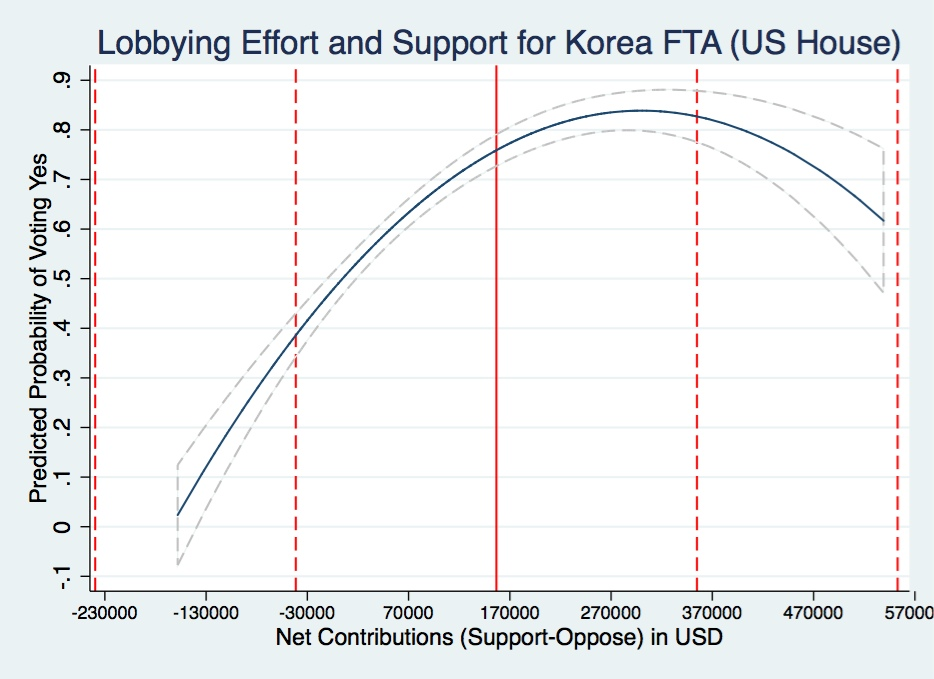
\includegraphics[height=2.75in, width=4.25in]{graph2.jpg}
%\end{frame}


\begin{frame}
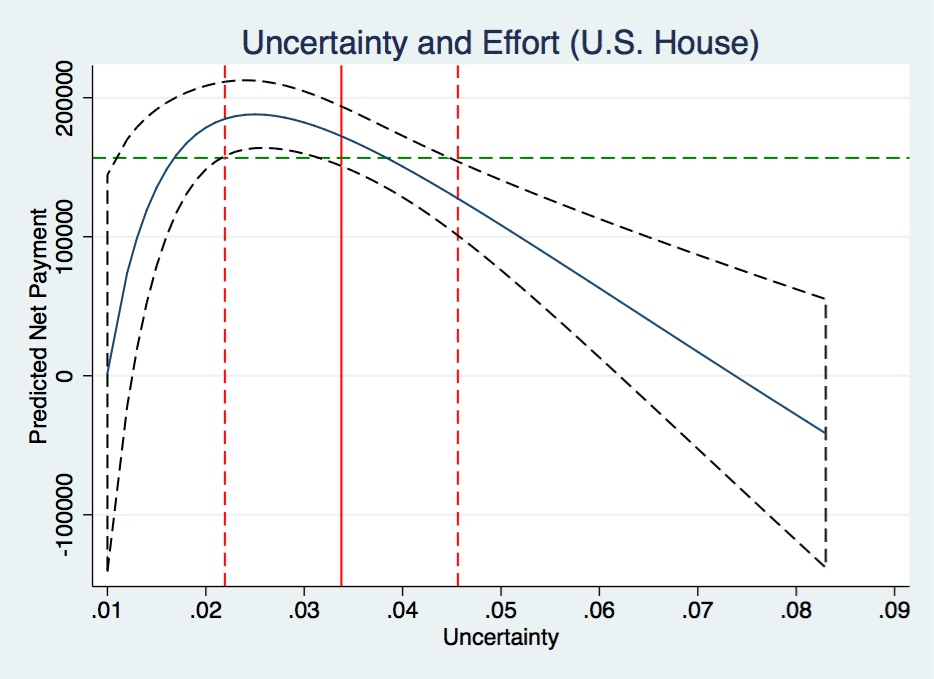
\includegraphics[height=2.75in, width=4.25in]{graph1.jpg}
\end{frame}


\begin{frame}{Preview}
\frametitle{Context}
\pause
U.S. House of Representative 
\pause
\begin{itemize}[<+->]
	\item All roll call votes, 2005 through present
	\item Interest group lobbying on each vote
	\item PAC contributions, LDA lobbying data
\end{itemize}

\vskip.2in
\pause
Goal: use multi-dimensional ideal-point estimation to identify measures of uncertainty
\end{frame}

\begin{frame}
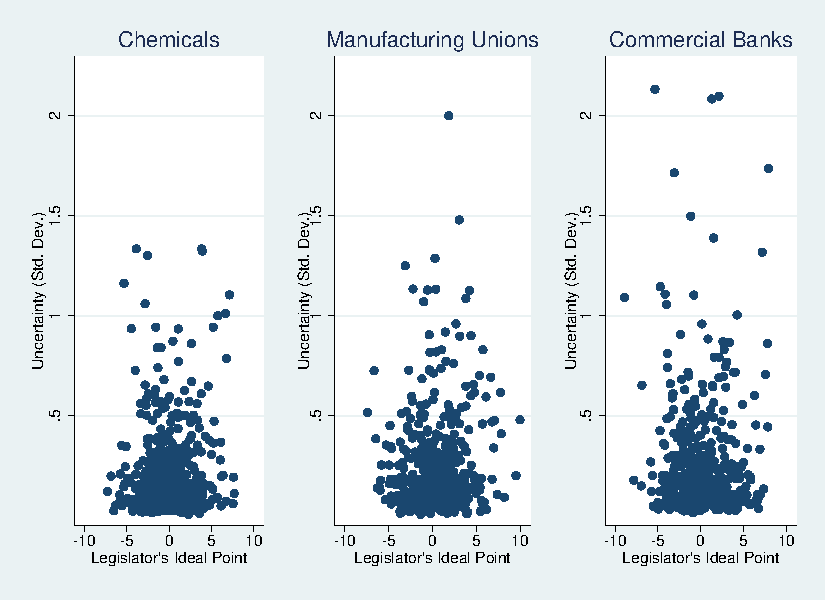
\includegraphics[height=2.75in, width=4.25in]{NSF_combined_graph.pdf}
\end{frame}





\section{Model}
\subsection{Political Structure}
\begin{frame}{Policy and Politics}

\pause
Two vote buyers, $A$ and $B$
\pause
\begin{itemize}
	\item A prefers $x$, $B$ prefers $s$
\end{itemize}

\pause
\vskip.2in
Three legislators
\pause
\begin{itemize}[<+->]
	\item Each will vote for status quo $\bm{s}$ or new proposal $\bm{x}$
	\item Decision made by majority vote
	\item Identified by location in linear preference space: $i \in \left\{-0.5,0,0.5\right\}$
		\begin{itemize}
			\item Take ideal point to be linear: $\alpha - \beta i$
		\end{itemize}
\end{itemize}


\end{frame}



\begin{frame}{Timeline}
\pause
\begin{enumerate}[<+->]
	\item {\bfseries Vote Buyer A}
		\begin{enumerate}[i.]
			%\pause
			\item Chooses bribes $\un{a} = \left(a_{-.5},a_0,a_{.5}\right)$
		\end{enumerate}
	%\pause
	\item \textbf{Vote Buyer B}
		\begin{enumerate}[i.]
			%\pause
			\item Observes $\un{a}$ (in sequential model)
			%\pause
			\item Chooses bribes $\un{b} = \left(b_{-.5},b_0,b_{.5}\right)$
		\end{enumerate}
	%\pause
	\item \textbf{Legislature}
	%\pause
		\begin{enumerate}[i.]
			\item All legislators observe $\un{a},\un{b}$
			\item Uncertainty about preferences realized: $\un{\ta} = \left(\ta_{-.5},\ta_0,\ta_{.5}\right)$
			\item Each legislator votes for her preferred policy 
		\end{enumerate}
\end{enumerate}
\end{frame}


\subsection{The Players}

\begin{frame}{Legislators}

\pause
Leg $i$ votes for $s$ if $v(i) = \alpha -\beta i + \ta_i + a_i - b_i \leq 0$
	\begin{itemize}[<+->]
		\item Probability $i$ votes for $s$ is
			\[ 
				\Pr\left[\alpha -\beta i + \ta_i + a_i - b_i \leq 0 \right]
			\]
			\[
				= \Pr\left[\ta_i \leq \beta i - \alpha - a_i + b_i \right]
			\]
		\item Assuming $\ta_i \text{ i.i.d.} \sim \text{Logistic} \ (0,1): \ = \frac{1}{1+e^{-\left(\beta i - \alpha - a_i + b_i \right)}}$ 
	\end{itemize}



\end{frame}


\begin{frame}{Vote Buyer B}
\pause
Assume vote buyers maximize expected value of winning net of bribes paid  
\pause
\begin{itemize}[<+->]
	\item Assume bribes must be non-negative
	\item Vote buyer won't spend more than his willingness to pay, $W_B$
	\item In three-seat legislature, maximize $[$ probability $\geq 2$ legislators vote for $s ]$ $\times W_B -$ bribes
\end{itemize}
\end{frame}

\begin{frame}{Vote Buyer B's Objective Function}
\pause
Let $S(i) = 1$ denote legislator $i$ votes for the status quo
\pause
\begin{multline*}
			    \max_{b_{-.5}, b_0, b_{.5}} 
					W_B \biggl[ \Pr\left(S\left(-.5\right)=1\right)\Pr\left(S\left(0\right)=1\right)\left(S\left(.5\right)=0\right)  + \\
					\Pr\left(S\left(-.5\right)=1\right)\Pr\left(S\left(0\right)=0\right)\Pr\left(S\left(.5\right)=1\right) + \\
					\Pr\left(S\left(-.5\right)=0\right)\Pr\left(S\left(0\right)=1\right)\Pr\left(S\left(.5\right)=1\right) + \\
					\Pr\left(S\left(-.5\right)=1\right)\Pr\left(S\left(0\right)=1\right)\Pr\left(S\left(.5\right)=1\right) \biggr] - \sum_{j\in \left\{-.5, 0,.5\right\}} b_j
				\end{multline*}
\end{frame}


\begin{frame}{Vote Buyer A}
\pause
Vote Buyer A is just like Vote Buyer B \textit{except}
\pause
\begin{itemize}[<+->]
	\item She gets to move first (in sequential model)
	\item She wants $x$ to win instead of $s$
	\item Willingness-to-pay parameter $W_A$
\end{itemize}
\end{frame}





\section{One Vote Buyer}
\subsection{}
\begin{frame}{Two Non-Negative Bribes}

\pause
Let $X$ and $Y$ and $Z$ be the gross positions of each of the three legislators. Then the FOCs are
\pause
	\begin{equation}
		\frac{e^{-Y} + e^{-Z}}{\left(1+e^{-Y}\right)\left(1+e^{-Z}\right)} \frac{e^{-X}}{\left(1+e^{-X}\right)^2}= \frac{1}{W_B}
	\end{equation}
	\begin{equation}
		\frac{e^{-X} + e^{-Z}}{\left(1+e^{-X}\right)\left(1+e^{-Z}\right)} \frac{e^{-Y}}{\left(1+e^{-Y}\right)^2}= \frac{1}{W_B}
	\end{equation}
	
\pause
\vskip.1in
\begin{beamerboxesrounded}[upper=palette tertiary, shadow=true]{Two non-negative bribes}
    When Vote Buyer $B$ pays bribes to exactly two legislators, the bribes are such that the two bribed legislators' ideal points gross of bribes are equalized. Which two legislators are bribed depends on the bias parameter $\al$.
\end{beamerboxesrounded}

\end{frame}


\begin{frame}{Three Non-Negative Bribes}
Similar intuition for the case where all three legislators are bribed
\pause
\vskip.4in
\begin{beamerboxesrounded}[upper=palette tertiary, shadow=true]{Three Non-Negative Bribes}
    When Vote Buyer $B$ pays bribes to all three legislators, the bribes are such that the legislators' ideal points gross of bribes are equalized.
\end{beamerboxesrounded}
\end{frame}

\begin{frame}{The Rest of the Story...}
\begin{beamerboxesrounded}[upper=palette tertiary, shadow=true]{One Non-Negative Bribe}
      When Vote Buyer $B$ pays bribes to exactly one legislator, it may be any one of the three legislators depending on the bias parameter $\al$.
\end{beamerboxesrounded}

\pause
\vskip.2in
\begin{beamerboxesrounded}[upper=palette tertiary, shadow=true]{No Non-Negative Bribes}
  When Vote Buyer $B$ has a low willingness to pay, he does not bribe any legislator.
\end{beamerboxesrounded}

\end{frame}


\begin{frame}{Varying Uncertainty Across Legislators}
Now let the scale of uncertainty differ across legislators 
\pause
\begin{itemize}[<+->]
	\item To be precise: the scale parameters in the three logit distributions are not equal
\end{itemize}

\pause
\vskip.2in
\begin{beamerboxesrounded}[upper=palette tertiary, shadow=true]{Conjecture}
 When there is no bias in the positions of the legislators ($\al =0$), the bribes of legislators whose ideal points are at the median in terms of uncertainty receive the highest relative bribes.\end{beamerboxesrounded}
\end{frame}

\section{Two Vote Buyers}
\subsection{Sequential Model}
\begin{frame}{Some Possibilities...}
\begin{beamerboxesrounded}[upper=palette tertiary, shadow=true]{No Bribes}
  It is possible that neither vote buyer bribes any legislator on a given vote. This occurs when both vote buyers' willingness-to-pay parameters are small.
\end{beamerboxesrounded}

\pause
\vskip.2in
\begin{beamerboxesrounded}[upper=palette tertiary, shadow=true]{Both Vote Buyers Bribe}
  It is possible for both vote buyers to bribe legislators on the same vote.
\end{beamerboxesrounded}

\end{frame}


\subsection{Simultaneous Model}
\begin{frame}{Some Possibilities...}
What I know...
\begin{itemize}
	\item FOCs look the same as for one vote buyer, e.g.
		\begin{equation*}
			\frac{e^{-Y} + e^{-Z}}{\left(1+e^{-Y}\right)\left(1+e^{-Z}\right)} \frac{e^{-X}}{\left(1+e^{-X}\right)^2}= \frac{1}{W_B}
		\end{equation*}
			\begin{itemize}
				\item Two roots, only larger one satisfies SOC
			\end{itemize}
\end{itemize}


\end{frame}


\section{Conclusion}

\begin{frame}{Next Steps}
\pause
\begin{itemize}[<+->]
	\item Modify model so that both legislators can lobby the \textit{same} legislator in equilibrium
	\item Derive tight identification of empirical estimates from structural model
	\item Provide micro-founded explanations for the variation in uncertainty that lobbies face
\end{itemize}

\end{frame}


\begin{frame}{Conclusion}
Taking into account uncertainty about the preferences of legislators brings vote buying models closer to capturing important stylized facts
\pause
\begin{itemize}[<+->]
		\item helps in understanding lobbying strategies
		\item may shed light on why some lobbies are more successful than others
		\item will help in the identification of measures of uncertainty that can be used in many applications
\end{itemize}

\end{frame}


\end{document}